%\documentclass[letterpaper, 10 pt, conference]{ieeeconf}
%\usepackage{filecontents,lipsum}
%\usepackage[noadjust]{cite}
%%\begin{filecontents*}{references.bib}
%%@article{Khoe:1994:CML:2288694.2294265,
%%    author = {Khoe, G. -D.},
%%    title = {Coherent multicarrier lightwave technology for flexible capacity networks},
%%    journal = {Comm. Mag.},
%%    issue_date = {March 1994},
%%    volume = {32},
%%    number = {3},
%%    month = mar,
%%    year = {1994},
%%    issn = {0163-6804},
%%    pages = {22--33},
%%    numpages = {12},
%%    url = {http://dx.doi.org/10.1109/35.267438},
%%    doi = {10.1109/35.267438},
%%    acmid = {2294265},
%%    publisher = {IEEE Press},
%%    address = {Piscataway, NJ, USA},
%%}
%%\end{filecontents*}
%\title{This document}
%\author{This author}

%%%%%%%%%%%%%%%%%%%%%%%%%%%%%%%%%%%%%%%%%%%%%%%%%%%%%%%%%%%%%%%%%%%%%%%%%%%%%%%%
%2345678901234567890123456789012345678901234567890123456789012345678901234567890
%        1         2         3         4         5         6         7         8

\documentclass[letterpaper, 10 pt, conference]{ieeeconf}  % Comment this line out if you need a4paper

%\documentclass[a4paper, 10pt, conference]{ieeeconf}      % Use this line for a4 paper

\IEEEoverridecommandlockouts                              % This command is only needed if 
                                                          % you want to use the \thanks command

\overrideIEEEmargins                                      % Needed to meet printer requirements.

% See the \addtolength command later in the file to balance the column lengths
% on the last page of the document

% The following packages can be found on http:\\www.ctan.org
%\usepackage{graphics} % for pdf, bitmapped graphics files
%\usepackage{epsfig} % for postscript graphics files
%\usepackage{mathptmx} % assumes new font selection scheme installed
%\usepackage{times} % assumes new font selection scheme installed
%\usepackage{amsmath} % assumes amsmath package installed
%\usepackage{amssymb}  % assumes amsmath package installed
%\usepackage{filecontents,lipsum}
%\usepackage[noadjust]{cite}
%\usepackage{bm}
%\usepackage{tikz}
%\usepackage{graphicx}
%\usepackage{caption}
%\usepackage{subcaption}
%\usepackage{multicol}
%\usepackage{url}
%\usepackage{geometry}
%\usepackage{mathtools}
%\usepackage[utf8]{inputenc}
%\usepackage[english]{babel}
%\usepackage{algorithm}
%\usepackage[]{algpseudocode}


\usepackage{afterpage}
\usepackage{algorithm}
\usepackage[]{algpseudocode}

\usepackage{stix}
\usepackage{amssymb}
\usepackage{amsmath}

\DeclareMathAlphabet\mathbfcal{OMS}{cmsy}{b}{n}
%\usepackage[math-style=TeX, bold-style=TeX]{unicode-math}

\usepackage{arydshln}
\usepackage[english]{babel}
\usepackage{bm}
\usepackage{caption}
\usepackage[T1]{fontenc}
\usepackage[]{graphicx}
\graphicspath{ {./fig/} }

\usepackage[utf8]{inputenc}
\usepackage{multicol}
\usepackage[T1]{xcolor}
\usepackage{soul}
\usepackage{subfig}
\usepackage{tikz}
\usepackage{url}
\usepackage[backend=biber,style=ieee,sorting=none]{biblatex}
\addbibresource{bib/references.bib}

\newcommand{\trsp}{{^{\top}}}

\newcommand\blankpage{%
    \null
    \thispagestyle{empty}%
    \addtocounter{page}{-1}%
    \newpage}



\newcommand*{\important}[1]{\textcolor{red}{\danger~\textbf{IMPORTANT:~}} \textcolor{red}{#1}}

\newcommand*{\pending}[1]{\textcolor{blue}{$\bigstar$~\textbf{PENDING~#1}}}

\newcommand\mybox[2][]{\tikz[overlay]\node[fill=blue!100,inner sep=4pt, anchor=text, rectangle, rounded corners=1mm,#1] {#2};\phantom{#2}}

\newcommand{\TODO}{\mybox[fill=yellow]{\textcolor{blue}{\Large \textbf{TODO}}}}
\newcommand\myhl[1]{\textcolor{red}{#1}}


\newtheorem{prop}{Proposition}

\title{\LARGE \bf
Dynamic sensorimotor graphs
}


\author{Some Guy, Random Stranger and Anonymous Dude}

\begin{document}

\maketitle

\begin{abstract}
Regularities present in the somatosensory signals of a robotic agent can reflect its embodiment and the associations resulting from the active control policy. In this work, we analyze the dynamic functional connectivity of the somatosensory signals based on the instantaneous pairwise mutual information. As the robot performs exploratory motions based on motor babbling, we capture and study the time-varying changes in the signal relationships. We analyze the instantaneous and average information sharing and associate them with different information states. Results from a simulated planar system validate using the instantaneous mutual information to extract and leverage the relationships between the somatosensory signals and defining exploratory motions related to self-touch events.
\end{abstract}
% =============================================================================
%                                                                             |
%                                                                             |
% ------------------------------- SECTION ------------------------------------|
%                                                                             |
%                                                                             |
% =============================================================================

\section{Introduction}\label{sec:intro}

The study of the structural and functional connectivity in the brain has furthered the understanding of its organizations and information processing. An analogy with the sensorimotor signals of an embodied agent is yet to be realized. While looking at the structural connectivity of the sensorimotor signals is difficult, studying their functional connectivity to extract information about the body structure and the emergence of behaviors based on information acquisition is undoubtedly realizable. The underlying premise is that regularities among the robot's sensorimotor signals connect tightly to the robot's embodiment. These regularities, known as \emph{sensorimotor contingencies} (SMC) \cite{Jacquey2019Sensorimotorcontingenciesas}, can be identified and studied using information-theoretic methods. This work explores an embodied agent's time-varying sensorimotor functional structure, leveraging information and graph theory concepts. 
% ---
\begin{figure}[!ht]
	\centering
	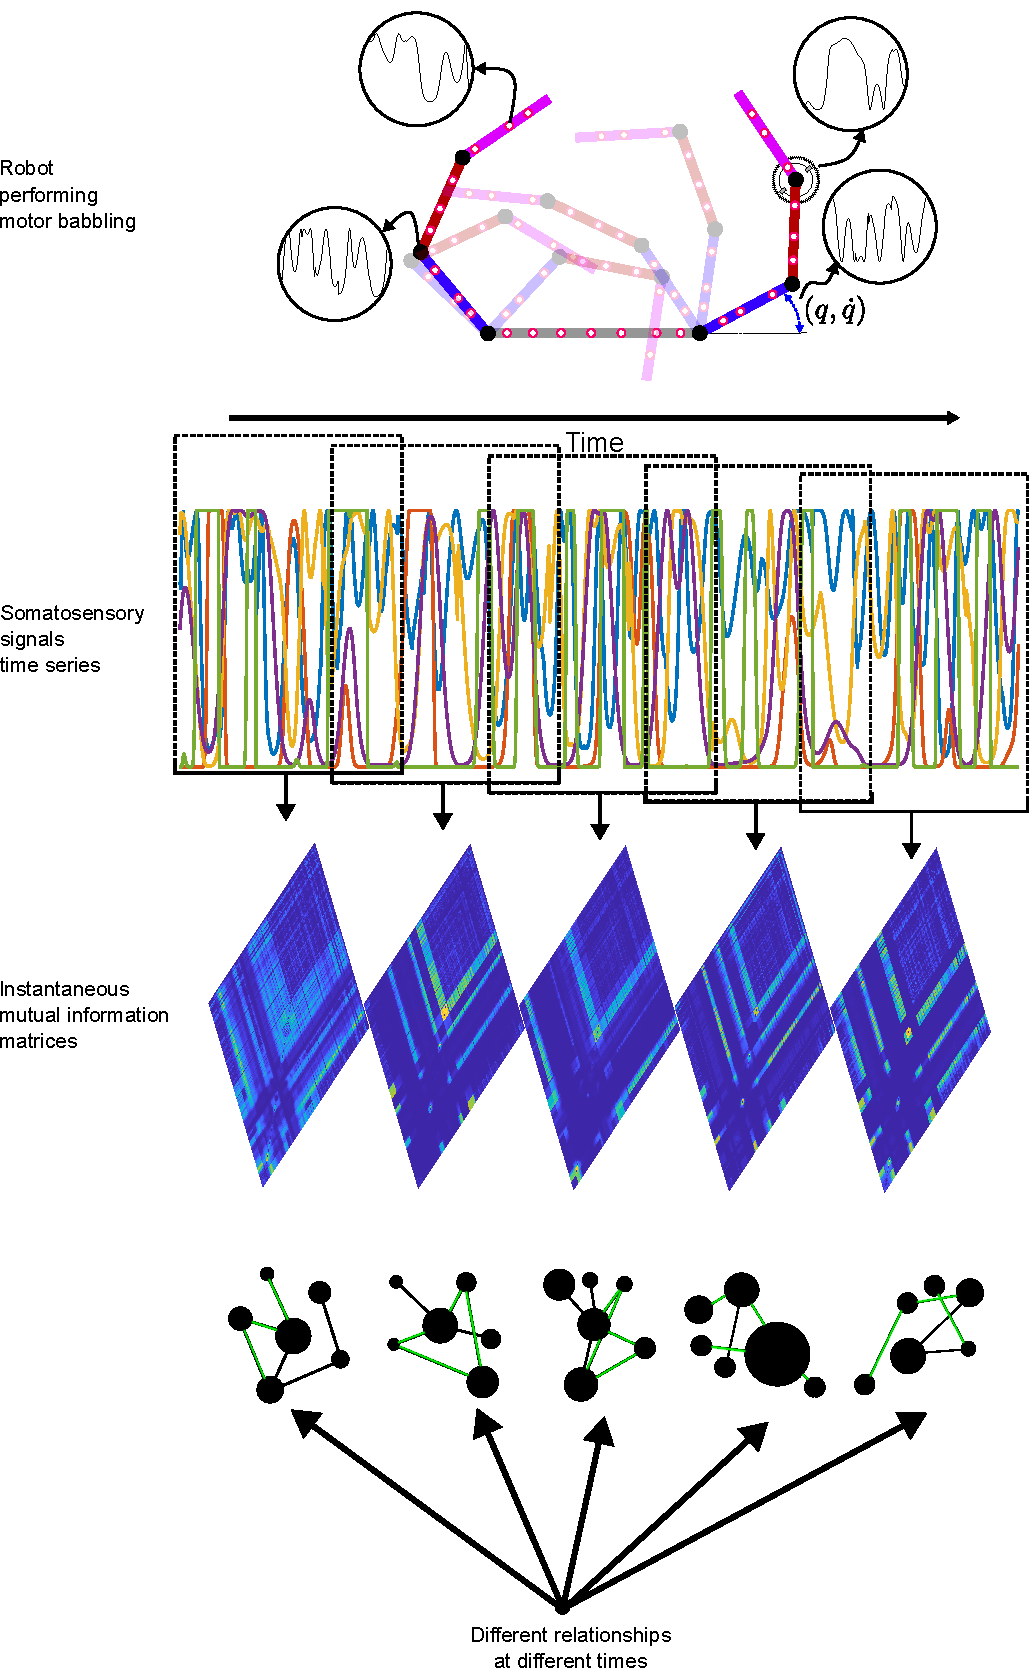
\includegraphics[width=0.9\columnwidth]{somatosensry_dynamic_functional_connectivity.pdf}
	\caption{General overview. While moving, the sensorimotor functional connectivity changes in time}
	\label{fig:general_overview}
\end{figure}
% ---
% SUBSECTION ==================================================================
\subsection{Related works}
%Some examples of previous works that have used information theory in this context include  \cite{Schmidt2013Bootstrappingperceptionusing,Lungarella2006Mappinginformationflow,Polani2009Modelsinformationprocessing,Bossomaier2016introductiontransferentropy,Olsson2006unknownsensorsactuators}. Although the literature about sensorimotor representations is extensive \cite{Nguyen2021Sensorimotorrepresentationlearning}, this work considers that the representation of SMCs as \emph{dynamic} graphs and their corresponding analysis aided by concepts from graph theory could provide further understanding about their formation and evolution. To achieve such a representation, methods from \emph{network topology inference} (NTI)\cite{Dong2019Learninggraphsdata} are regarded to study the relationships among the different constituent elements of the graph.

As established in \cite{Jacquey2019Sensorimotorcontingenciesas}, SMCs play a role in acquiring body knowledge, generalization, and goal-directedness. Yet, although the literature about sensorimotor representations is extensive \cite{Nguyen2021Sensorimotorrepresentationlearning}, the connections between sensorimotor regularities and body knowledge are poorly understood. Several works \cite{Schmidt2013Bootstrappingperceptionusing,Lungarella2006Mappinginformationflow,Polani2009Modelsinformationprocessing,Bossomaier2016introductiontransferentropy,Olsson2006unknownsensorsactuators} have used information-theoretic metrics to study these relationships in the sensorimotor system. Additionally, when exploring SMCs, touch is an essential sensory modality. For example, the work by \cite{Gama2021Goaldirectedtactile} discussed using intrinsic motivation and goal-babbling for learning self-touch on a simulated humanoid robot with artificially sensitive skin. Self-touch for calibration was used in \cite{Roncone2014Automatickinematicchain}, letting the robot close the kinematic chain by touching its own body. In \cite{Marcel2022Learningreachown}, a multimodal variational autoencoder in a denoising framework is used to learn the latent representation of self-touch that allows the agent to reconstruct self-reaching configurations internally.
%These works \myhl{The paper contributes to the sensorimotor contingency theory by providing a computational model that supports the hypothesis that the representation of self-touch can be learned simply through self-exploration.}

The study of functional connectivity has shown that the statistical properties of the considered signals and their relationships may vary over time. This \emph{dynamical} functional connectivity (DFC) has mainly been used to study functional networks in the brain to, for example, show states of lower functional connectivity during onsets of epilepsy\cite{Christiaen2020Dynamicfunctionalconnectivity} or identify potentially abnormal connectivity patterns in The work in brains affected by illness\cite{Zhou2020Earlychildhooddevelopmental}. Recently it was used to identify evolving relationships in the sensorimotor signals of a simulated infant based on age \cite{Kanazawa2023Openendedmovements}. %In robotics, it is expected that depending on the motion policy driving the robot or the task being executed by it, the sensorimotor connectivity will also change. 

% SUBSECTION ==================================================================
\subsection{Contributions}
This work considers that representing the functional connections between somatosensory signals (touch and proprioception) of an embodied agent as \emph{dynamic} graphs and their corresponding analysis can help understand the formation and evolution of SMCs. Given that, based on the motion policy driving the robot or the task it executes, sensorimotor connectivity will also change, capturing and studying these varying connectivity patterns is essential. We achieve this by looking at the instantaneous mutual pairwise mutual information showing how the state of information sharing in the system is related to its motion and potential interactions with itself. Using non-negative matrix factorization, we identify different information-sharing states and classify them according to their information content. In a case study, we demonstrate how, after a motor babbling phase, by only focusing on the mutual information and without knowing the robot's morphology, an excitation trajectory for both the robot arms can be devised that avoids self-contact. A comparison of this trajectory against conventional trajectory design methods is presented.

% =============================================================================
%                                                                             |
%                                                                             |
% ------------------------------- SECTION ------------------------------------|
%                                                                             |
%                                                                             |
% =============================================================================
\section{The embodied agent}

% SUBSECTION ==================================================================
\subsection{The planar dual arm model}
We use as a reference system the robot model presented in \cite{Mannella2018Knowyourbody,Marcel2022Learningreachown}, consisting of a simple six degrees-of-freedom planar dual arm system with three links per arm and a fixed torso, see Fig.~\ref{fig:extended_dual_arm_robot}. The robot is equipped with a set of tactile sensors distributed along the robot's body. The dynamics of the model were instantiated by assigning inertial properties to the robot's composing bodies. Its actuation mechanism is based on the biology-inspired model presented in \cite{Ekeberg1993combinedneuronalmechanical,Wadden1998neuromechanicalmodel, Shim2012Chaoticexplorationlearning}, where each joint is driven by antagonistic muscles (modeled as spring-damper systems) whose pulling force is linearly controlled by the signal of a corresponding motor neuron $\sigma$. The generated joint torque, expressed as
% ---
\begin{equation}\label{eq:antagonistic_torque}
	\tau = \alpha \left(\sigma_{fx} - \sigma_{ex}\right)  + \beta \left(\sigma_{fx} + \sigma_{ex} + \gamma \right) q + \delta \dot{q},
\end{equation}
% ---
results from the difference between the flexion $ \sigma_{fx} $ and extension $\sigma_{ex}$ activation signals which create the flexion and extension pulling forces $ f_{fx}$ and $f_{ex} $. The parameters are:
% ---
\begin{itemize}
	\item $\alpha$: muscle force gain
	\item $\beta$: stiffness gain
	\item $\gamma$: tonic stiffness	
	\item $\delta$: damping coefficient
\end{itemize}

% SUBSECTION ==================================================================
\subsection{The set of somatosensory signals}
The tactile sensors on the robot's body are modeled based on population coding \cite{Panzeri2010PopulationCoding} represented as distance-dependent Gaussian receptive fields (see Fig.~\ref{fig:population_coding}), with the location of the sensors (randomly located along the robot's one-dimensional body) being the means of the receptive fields. We modified the tactile sensors to account for the strength of touch. Essentially, the previously distance-based activation of the Gaussian receptive fields is now scaled by the contact force. Similar to the tactile sensors, the robot's proprioceptive measurements are also encoded using receptive fields. Therefore, the vector of somatosensory signals $\bm{s}$ in the extended model consists of proprioception that encompasses joint position $\bm{p}$, velocity $\bm{v}$, and effort $\bm{e}$, as well as touch signals $\bm{r}$ (scaled by the touch force); i.e.:
% ---
\begin{equation}
	\bm{s} = \begin{bmatrix}
		\bm{p}\trsp & \bm{v}\trsp & \bm{e}\trsp & \bm{r}\trsp
	\end{bmatrix}\trsp \in \mathbb{R}^{N_s}_{\geq}
\end{equation}
%---
%\begin{figure*}[htp!]
%	\centering	
%	\hspace*{\fill}
%	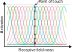
\includegraphics[width= 0.6\textwidth]{fig/receptive_fields.pdf}
%	\hspace*{\fill}
%	\caption[] {\label{fig:receptive_fields} The Gaussian receptive fields used in population coding.}
%\end{figure*}
% ---
\begin{figure}[!t]
	\begin{center}
		\hspace*{\fill}
		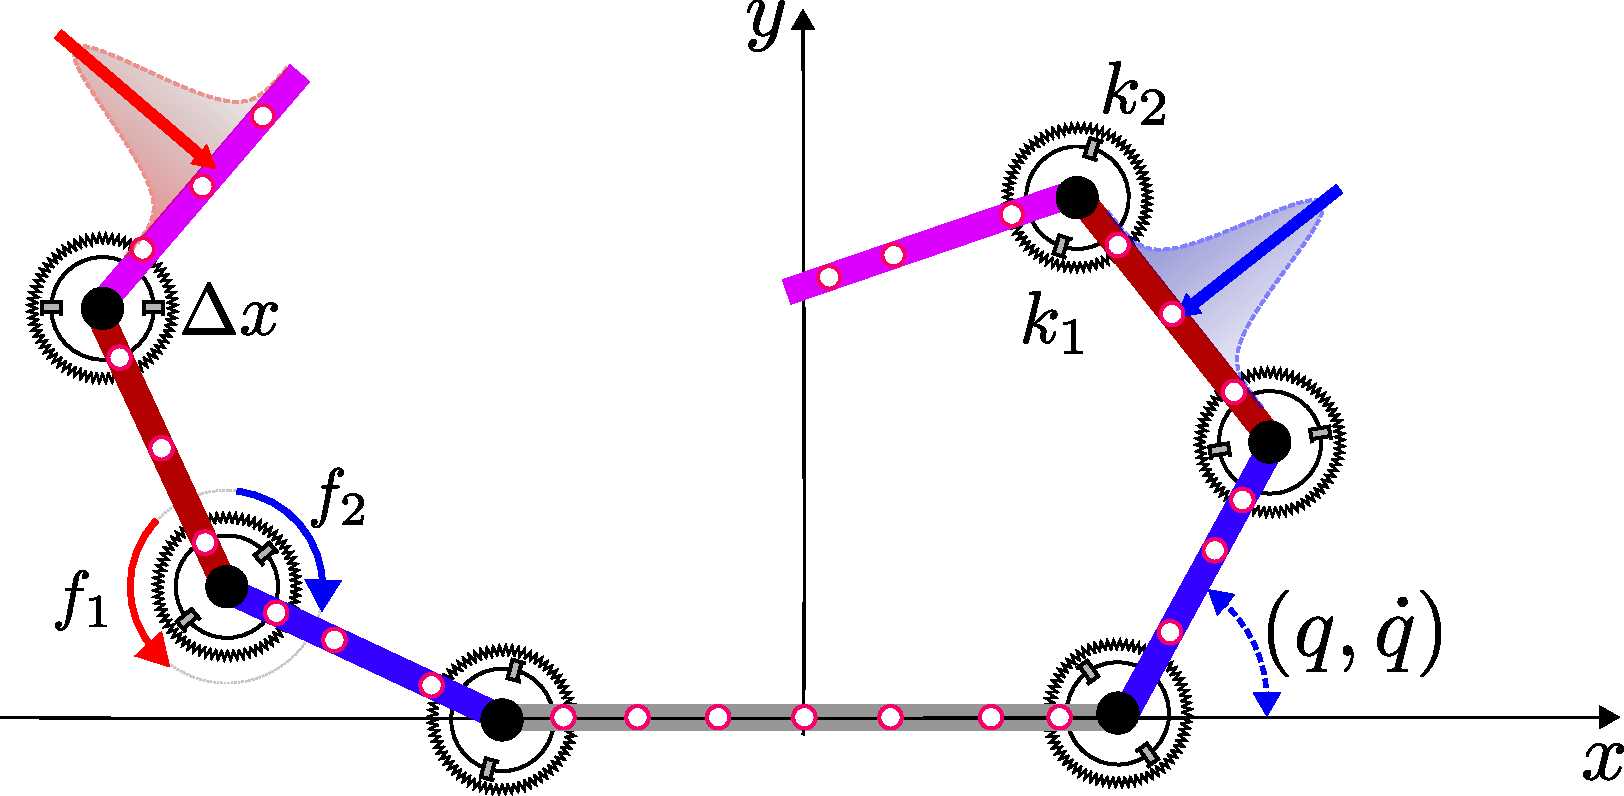
\includegraphics[width=0.99\columnwidth]{extended_dual_arm_robot.pdf}
		\hspace*{\fill}
	\end{center}
	\caption{\label{fig:extended_dual_arm_robot} The planar dual arm robot with antagonistic actuation.}
\end{figure}
% ---


% ---
\begin{figure}[!t]
	\begin{center}
		\hspace*{\fill}
		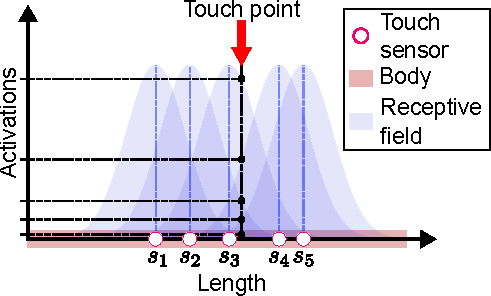
\includegraphics[width=0.99\columnwidth]{touch_receptive_fields.pdf}
		\hspace*{\fill}
	\end{center}
	\caption{\label{fig:population_coding} The receptive fields used in population coding.}
\end{figure}
% ---
% =============================================================================
%                                                                             |
%                                                                             |
% ------------------------------- SECTION ------------------------------------|
%                                                                             |
%                                                                             |
% =============================================================================
\section{The sensorimotor dynamic functional connectivity}

% Subsection ==================================================================
\subsection{Functional connectivity}
%Finding and graphically representing the relationships among the constituent elements of a system is known as \emph{network topology inference} (NTI) \cite{Dong2019Learninggraphsdata}. By learning the topology of a network (also known as a graph), it is possible to reveal a structure that aids in the analysis of the interaction among the entities. When relying only on measurement signals to estimate the network topology, approaches based on physically-motivated and statistical models are typically used\cite{Dong2019Learninggraphsdata}. In particular, the latter entails methods based on correlation, probabilistic graphical models, entropy, mutual information, and transfer entropy. Recently, other methods for NTI have been provided within the framework of Graph Signal Processing (GSP) \cite{Stankovic2019Introductiongraphsignal,Dong2019Learninggraphsdata,Mateos2019ConnectingdotsIdentifying}. Exemplary works showing the representation and analysis possibilities brought about by NTI include \cite{Zhang2017Networkbasedmachine,Karwowski2019Applicationgraphtheory,Sporns2018Graphtheorymethods}. 

\emph{Functional connectivity} (FC) is a method for network topology inference that characterizes the dependencies of the observed signals from a system based on their probability distributions\cite{Friston2011Functionaleffectiveconnectivity}. It can be subdivided into undirected and directed; the latter being related to the analysis of statistical causation from the data \cite{Bastos2016tutorialreviewfunctional}. By studying the FC  it is possible to reveal a structure that aids in the analysis of the interaction among the entities.

Based on the connection between embodiment and information structure \cite{Pfeifer2007Selforganizationembodiment}, our hypothesis is that properties of the sensorimotor interactions can be made apparent by studying the FC among the somatosensory signals $ \bm{s}(t) $. From the various metrics that have been proposed to evaluate such relationships, we, in particular, leverage those based on information theory \cite{Bonsignorio2020EntropyBasedMetrics,Bonsignorio2013Quantifyingevolutionaryself}, as their \emph{model-free} nature can capture linear and nonlinear relationships between signals. Particularly, we use the \emph{mutual information} (MI), a quantity that has been applied in different contexts to quantify the relationships between variables \cite{Steuer2002mutualinformationdetecting}. The MI between two signals $ I\left(X;Y\right) $ can be interpreted as the amount by which a random signal $ Y $ reduces the uncertainty about a random signal $ X $ \cite{Cover1999Elementsinformationtheory}. It is a symmetric measure of the information sharing by both signals and is computed as:
% ---
\begin{equation}\label{eq:mutual_information}
	I\left(X;Y\right) =I\left(Y;X\right) = H(X) + H(Y) - H(X,Y)
\end{equation}
% ---
with the Shannon's entropy of a variable $X$ defined by 
% ---
\begin{equation}\label{eq:entropy}
	H(X) = -\sum_{i=1}^{n}p(x_i)\text{log}_2\left(p\left(x_i\right)\right)
\end{equation}
% ---
and the joint entropy between $ X $ and $ Y $ expressed as
% ---
\begin{equation}\label{eq:joint_entropy}
	H(X,Y) = -\sum_{i=1}^{n}\sum_{j=1}^{n} p(x_i,y_j)\text{log}_2\big(p\left(x_i,y_j\right)\big).
\end{equation}
% ---
By extension, the mutual information matrix $\bm{\mathcal{I}} \in \mathbb{R}^{m \times m}$ can be constructed by computing the pairwise MI between the $\left\lbrace s_i\right\rbrace^{N_s}_{i=1}$ somatosensory signals. Its $(i,j)$ entries are given by
% ---
\begin{equation}\label{eq:adjacency_mi}
	(\bm{\mathcal{I}})_{i,j} = I(s_i;s_j).
\end{equation}
% ---
In practice, computing \eqref{eq:adjacency_mi}  for a pair $\left({s}_i(t),{s}_j(t)\right)$ involves centering their samples (to zero mean and unit standard deviation) and using either binning, kernel, or nearest neighbor methods \cite{WaltersWilliams2009Estimationmutualinformation} to compute their mutual information. In this work, for the computation of $\bm{\mathcal{I}}$, we use the open-source MATLAB package \emph{Mutual information computation}\cite{PengMutualInformationcomputation}.

% Subsection ==================================================================
\subsection{Dynamic functional connectivity}
When analyzing FC, it might be interesting to look at the aggregated effect of a complete dataset of recordings and the instantaneous changes that occur in the relationships. Indeed, the functional relationships between sensorimotor signals can change rapidly depending on the motion policy and the interaction of the agent with the environment. To capture this time-varying, i.e., \emph{dynamic}, functional connectivity with mutual information, it is common to use a sliding time window \cite{Preti2017dynamicfunctionalconnectome} with forward step $\Delta t$ from which the MI is computed only for a small number of samples.

In particular, for a time window of length $T$. The mutual information $I_t(s_x(t);s_y(t))$ for a distinct pair of signals $s_x(t)$ and $s_y(t)$ at time $t$ is computed for the set of signal samples spanning the interval $\left[t-T,t\right]$, see Fig.~\ref{fig:mi_sliding_window_mi}. We called this term the \emph{instantaneous mutual information} (IMI). It follows that the mutual information matrix $\bm{\mathcal{I}}(t)$ at time $t$ is constructed by computing the IMI for all the pairwise signals in the same time interval. The time series the time-varying mutual information matrix $\bm{\mathcal{I}}(t)$ shows the dynamical functional connectivity between the somatosensory signals.
%In particular, as tactile events can occur in a short time scale, the mutual information was computed for a time window of length $T$. For any two distinct pair of signals $s_x(t)$ and $s_y(t)$, the mutual information $I_t(s_x(t);s_y(t))$ at time $t$  is computed in the interval $\left[t-T,t\right]$, see Fig.~\ref{fig:mi_sliding_window_mi}. We called this term the \emph{instantaneous mutual information} (IMI). The forward step for the sliding window is $\Delta t$. The mutual information matrix $\bm{\mathcal{I}}(t)$ at time $t$ is constructed by computing the IMI for all the pairwise signals. Given a data matrix of somatosensory signals a time series the time-varying mutual information matrix $\bm{\mathcal{I}}(t)$ defines a expresses the dynamical functional connectivity between the signals.


% ---
\begin{figure}[!th]
	\begin{center}
		\hspace*{\fill}
		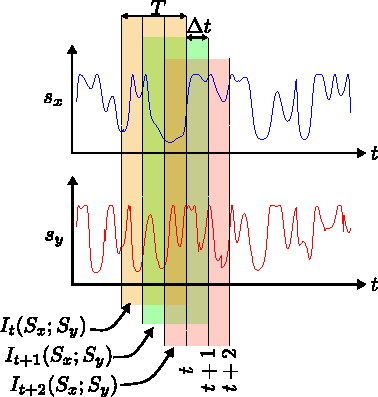
\includegraphics[width=0.99\columnwidth]{sliding_window_mi.pdf}
		\hspace*{\fill}
	\end{center}
	\caption{\label{fig:mi_sliding_window_mi} Sliding window strategy to compute the instantaneous mutual information.}
\end{figure}
% ---

\begin{figure}[!th]
	\centering
	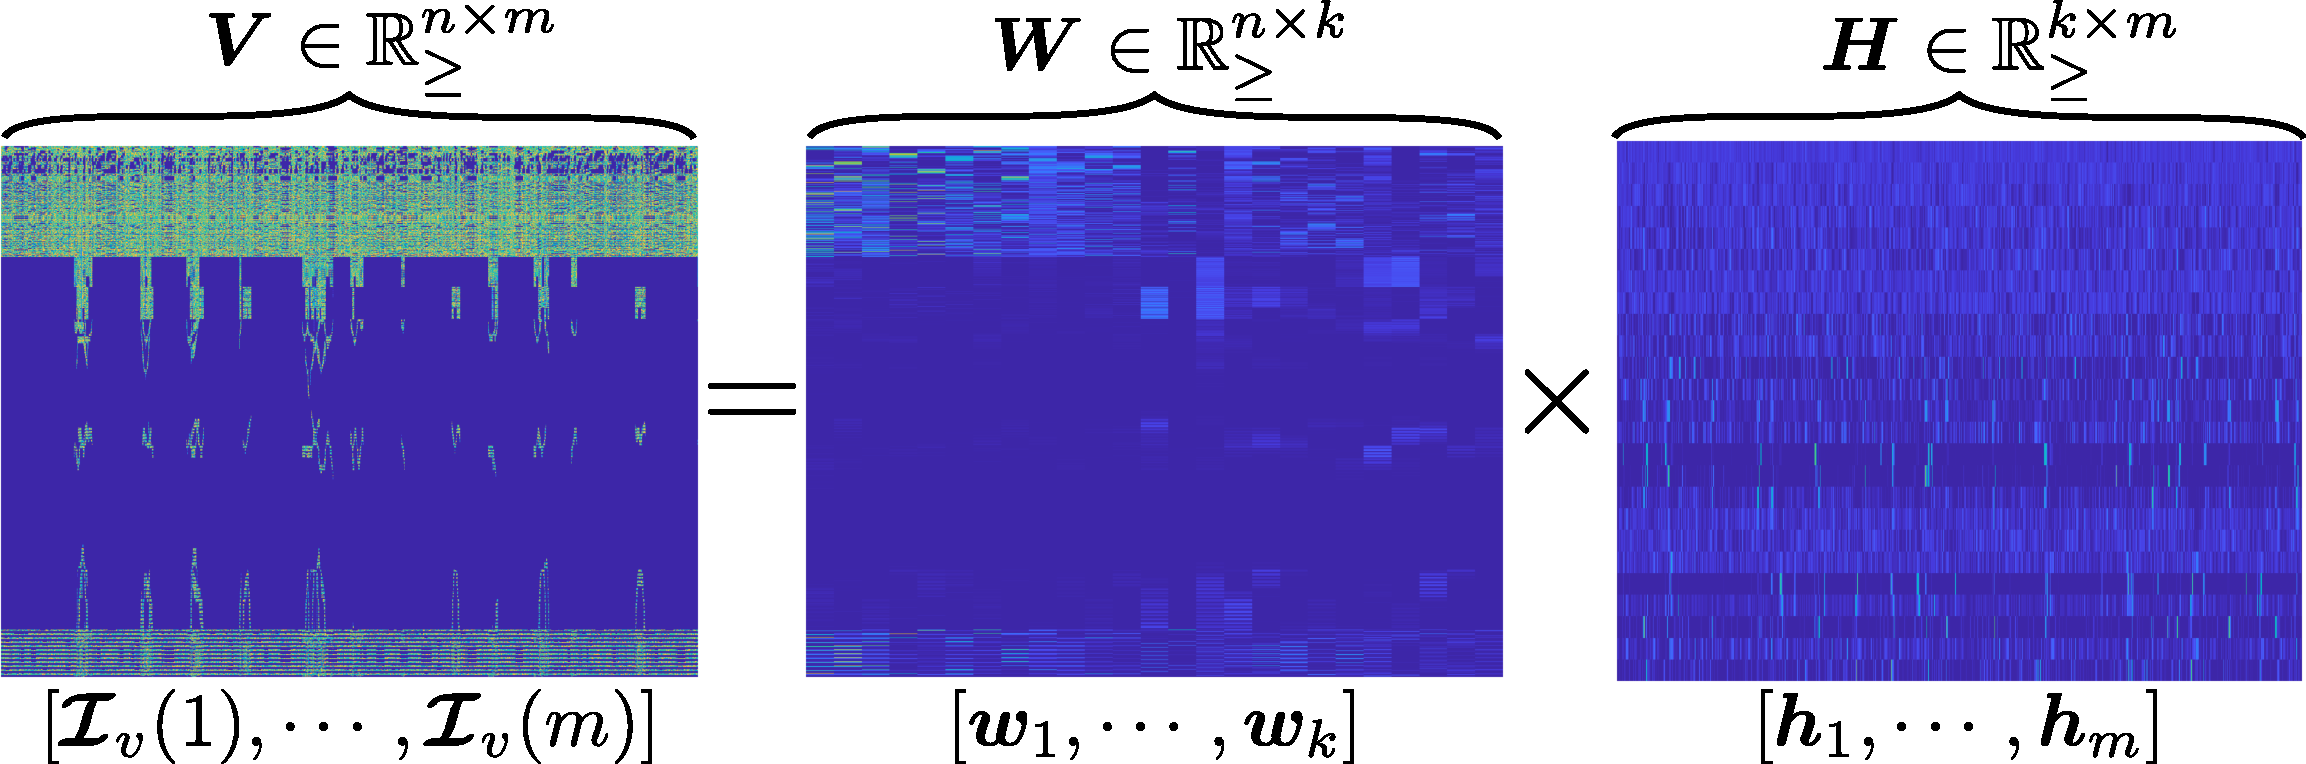
\includegraphics[width=0.99\columnwidth]{fig/nnmf_concept.pdf}
	\caption{Decomposition of the mutual information data matrix using non-negative matrix factorization.}
	\label{fig:nnmf}
\end{figure}

% Subsection ==================================================================
\subsection{Analyzing patterns}
Given a set of $m$ samples from the somatosensory signals generated, for example, via motor babbling, a dataset $\bm{S} \in \mathbb{R}^{n \times m}_{\geq}$ can be used to search for repeating patterns of FC that encode certain modes of operation. It is also important to determine these patterns' strength and frequency of expression to determine their relevance. Typical methods to detect repeating patterns in dynamic FC include the cosine similarity \cite{Menon2019comparisonstaticdynamic}, k-means clustering\cite{Li2017Hightransitionfrequencies}, and  non-negative matrix factorization (NNMF) \cite{Fu2019Nonnegativematrixfactorization}. We chose the latter, as it has proven useful in several studies analyzing brain dynamic functional networks and has also been used for community  detection\cite{Wang2011Communitydiscoveryusing,Luo2021Symmetricnonnegativematrix}.

NNMF is an unsupervised machine learning algorithm that can be used to split an input matrix $\bm{D}_{\bm{\mathcal{I}}} \in \mathbb{R}^{n\times m}_{\geq}$ into two parts: a matrix $\bm{W} \in \mathbb{R}^{n\times k}_{\geq}$ of bases and a matrix $\bm{H} \in \mathbb{R}^{k\times m}_{\geq}$ of their corresponding contributions to the input matrix $\bm{D}_{\bm{\mathcal{I}}}$; i.e.,
% ---
\begin{equation}
	\bm{D}_{\bm{\mathcal{I}}} 	\approx \bm{W} \bm{H}.
\end{equation}
% ---

In our case, the matrix $\bm{D}_{\bm{\mathcal{I}}}$ is constructed by vectorizing  and concatenating each of the matrices $\bm{\mathcal{I}}_v(t) = \text{vec}\left(\bm{\mathcal{I}}(t)\right)$; that is: 
\begin{equation}
	\bm{D}_{\bm{\mathcal{I}}} = [\bm{\mathcal{I}}_v(1),\cdots,\bm{\mathcal{I}}_v(m)]
\end{equation}
Note that $n = N_s(N_s-1)/2$ is the total number of mutual information pairs. Since the matrix $D_{\bm{\mathcal{I}}}$ is strictly non-negative, it is straight away suitable for its decomposition and analysis using NNMF. One crucial question is the number of factors $k$ used to approximate the original dataset. From the various methods to select an adequate number \cite{Muzzarelli2019RankSelectionNon}, we chose $k$ following the elbow method as in \cite{Phalen2020Nonnegativematrix} by performing NNMF for ascending values of $k$ and selecting the value where the residual error is not reduced any further.

Each of the factors $\left\lbrace\bm{w}_i\right\rbrace^k_i=1$ can be interpreted as a base FC graph capturing
a state of information sharing of multiple sensorimotor states. When the factors are aggregated using via the columns of $\bm{H}$, the particular mutual information matrix at time $t$ is closely approximated.

%It is worth mentioning that NNMF is an stochastic method and thus, two different runs will produce two distinct set of factors. 
To facilitate the analysis of the relevance of each of the factors, after factorization, the factors are normalized according to the $L_2$-norm. 

% XXXXXXXXXXXXXXXXXXXXXXXXXXXXXXXXXXXXXXXXXXXXXXXXXXXXXXXXXXXXXXXXXXXXXXXXXXXXXX
%Intuitively, NMF decomposes functional brain networks into the following: (1) a set of subnetworks (patterns) overlapping in space and
%time and (2) corresponding coefficient time series that quantify the
%contribution of each subnetwork (pattern) at each time point
%(Chai et al., 2017; Khambhati et al., 2017, 2018a,b). 
%
%As compared to
%hard-partitioning schemes, the advantage of this method is that it
%provides information about brain-network dynamics in a continuous,
%overlapping manner in space and time rather than in discrete partitions.
%Furthermore, owing to the parts-based nature of the technique, we
%obtained subnetworks that resembled the localized features of largescale brain networks rather than generalized patterns of the overall
%network
% XXXXXXXXXXXXXXXXXXXXXXXXXXXXXXXXXXXXXXXXXXXXXXXXXXXXXXXXXXXXXXXXXXXXXXXXXXXXXX

%In \cite{Stiso2020Learningbraincomputer} it is shown how the basis graph change their expressing during learning of a task



% =============================================================================
%                                                                             |
%                                                                             |
% ------------------------------- SECTION ------------------------------------|
%                                                                             |
%                                                                             |
% =============================================================================
\section{Simulation results}

% ---
\begin{figure}[!th]
	\begin{center}
		\hspace*{\fill}
		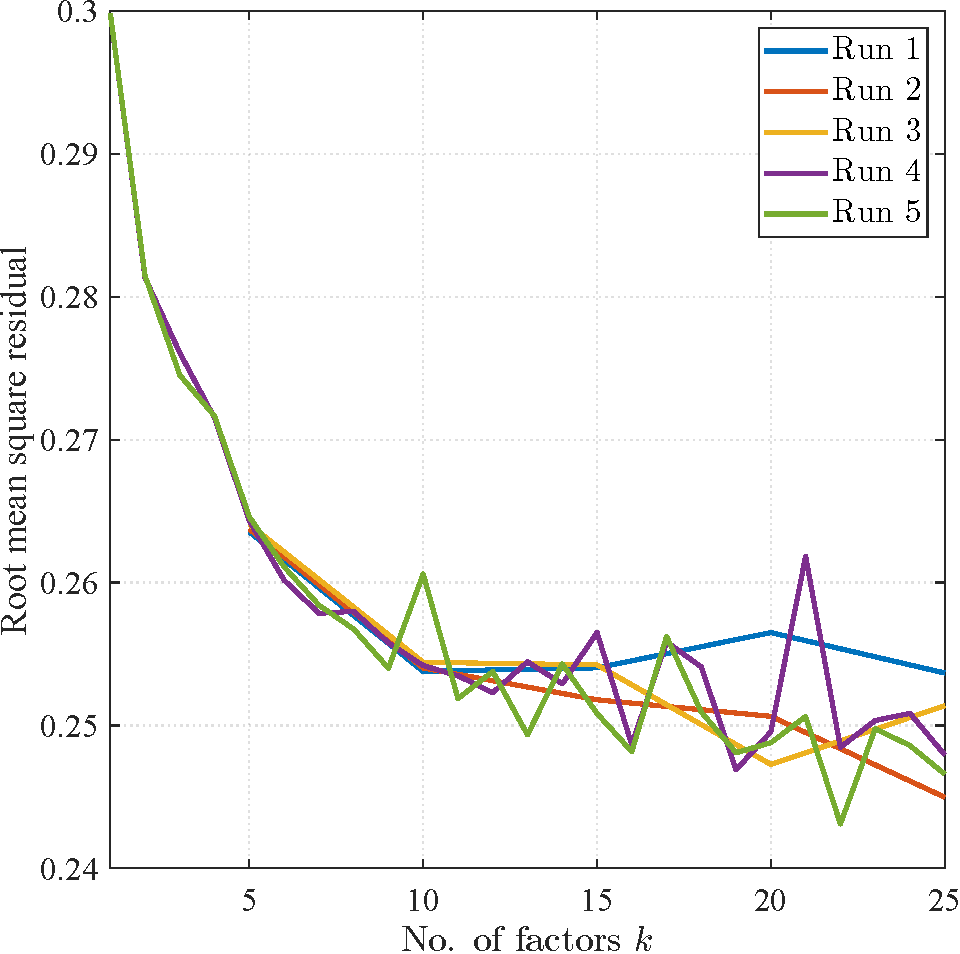
\includegraphics[width=0.99\columnwidth]{nnmf_elbow.pdf}
		\hspace*{\fill}
	\end{center}
	\caption{\label{fig:nnmf_elbow} Elbow method to determine the number of factors for NNMF.}
\end{figure}
% ---

\subsection{Exploratory phase}
\begin{figure*}[!ht]
	\centering
	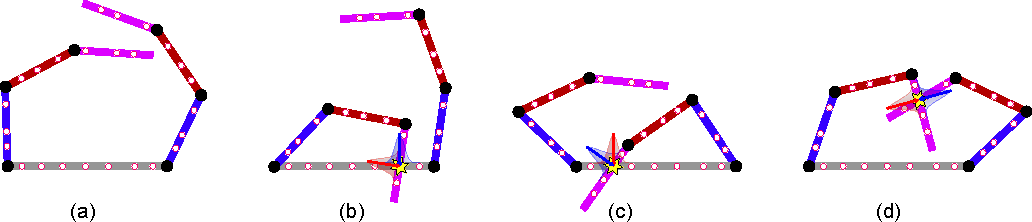
\includegraphics[width=0.9\textwidth]{planar_dual_arm_modes.pdf}
	\caption{Different events during exploration. (a) Pure proprioception (no touch), (b) contact with left arm, (c) contact with right arm, and (d) contact with both arms.}
	\label{fig:planar_dual_arm_modes}
\end{figure*}
% ---
For the computation of the instantaneous mutual information, we used sensor signals sampled at 100 Hz and a sliding window of $T = 0.1$ seconds, i.e., the previously seen 10 samples. With this short memory which is stored in a buffer, we can capture (fast) touch events.

% Subsection ==================================================================
\subsection{Dimensionality reduction}
To show graphically how the different factors cluster naturally depending on the touched regions, we used the PaCMAP dimensionality reduction method \cite{Wang2021Understandinghowdimension} given its properties to preserve aspects of the global and local structure when reducing into the latent space \cite{Huang2022Towardscomprehensiveevaluation}.

\begin{figure}[!th]
	\centering
	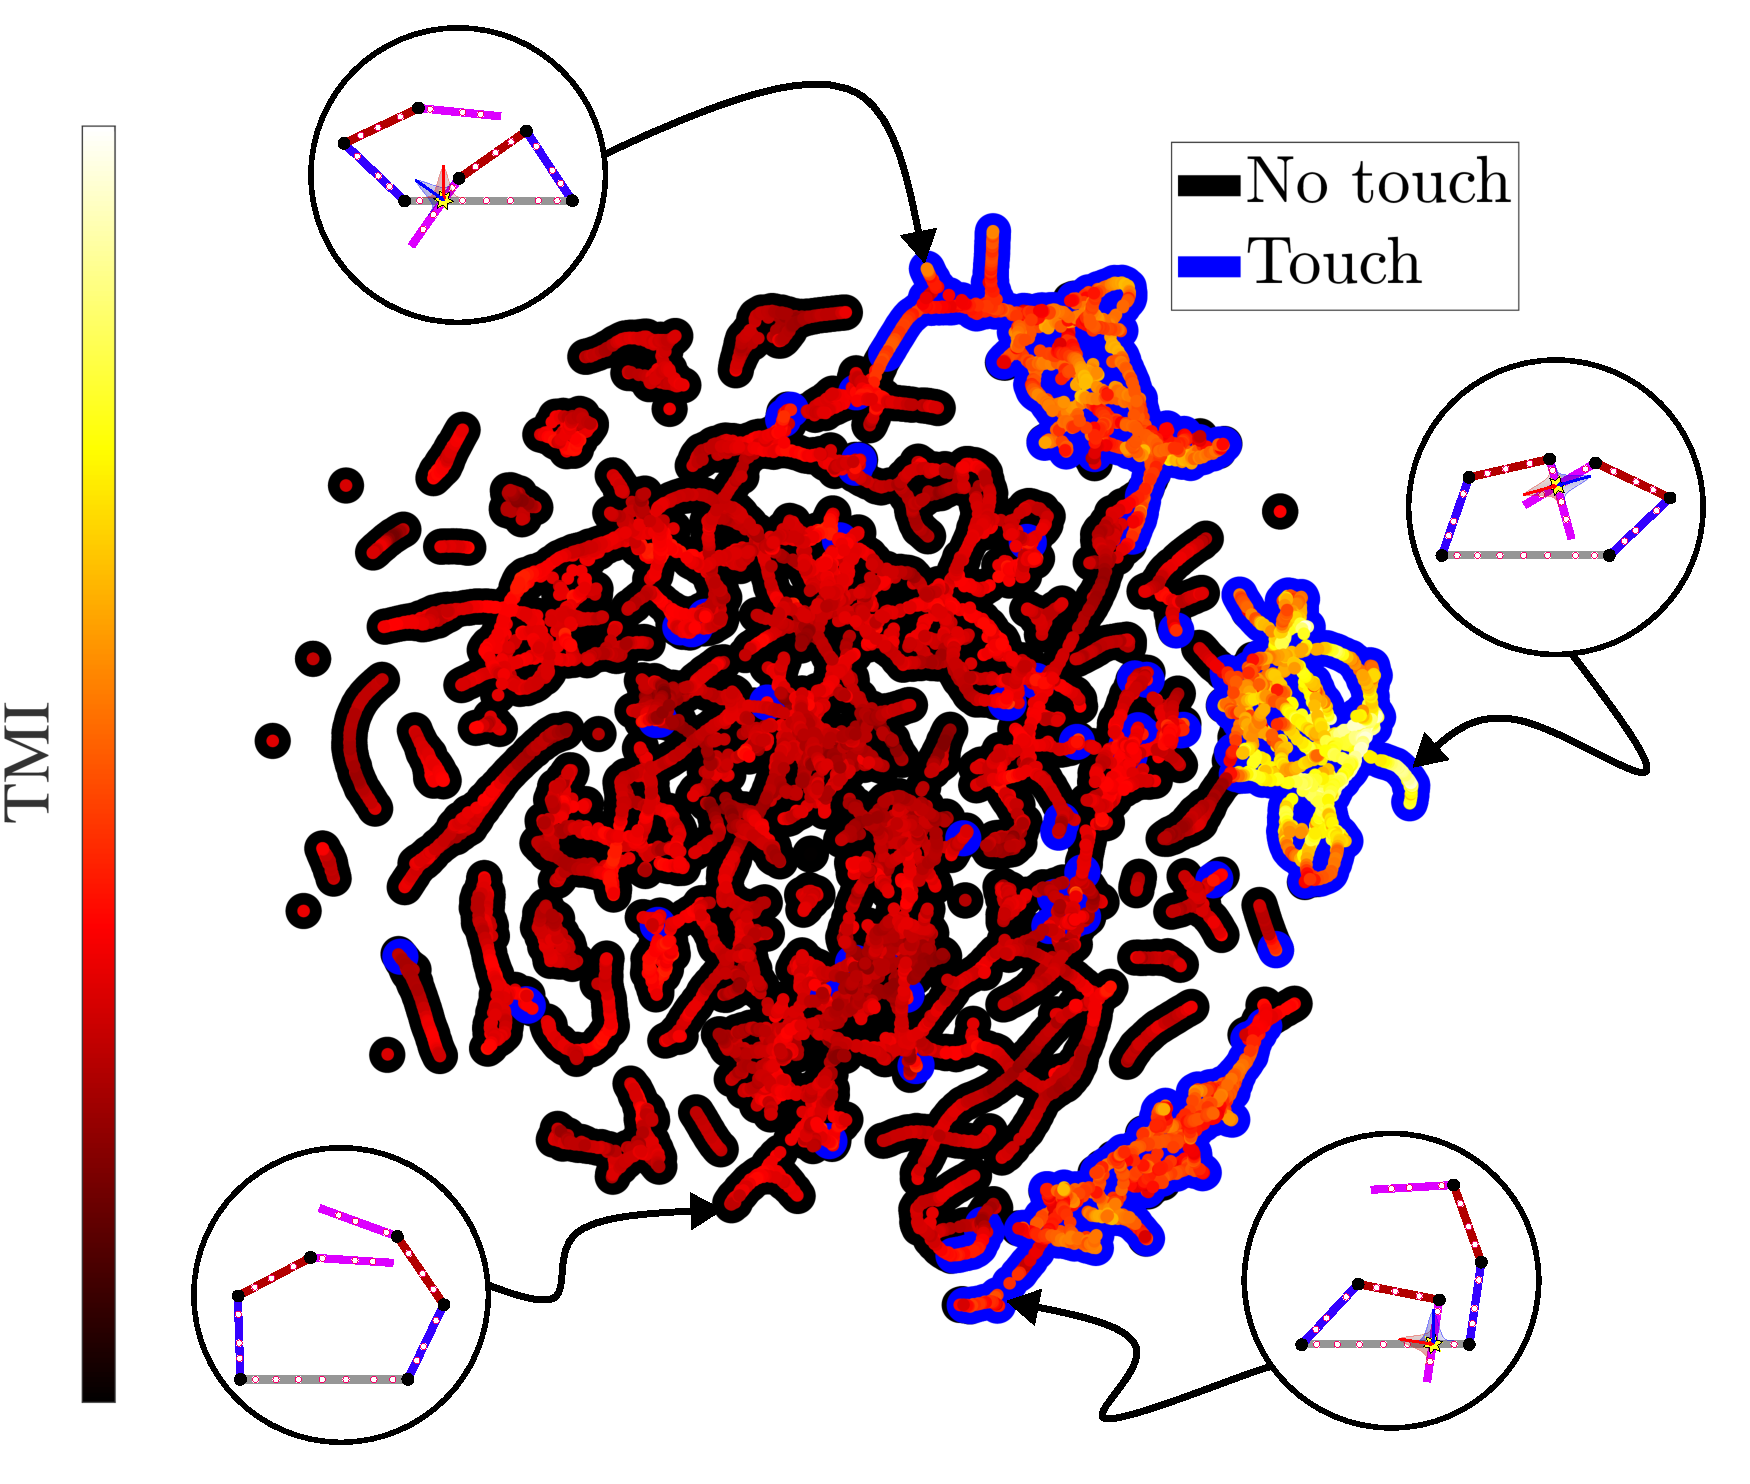
\includegraphics[width=0.99\columnwidth]{fig/pacmac_with_timi_and_modes.pdf}
	\caption{A two dimensional projection using PaCMAP of the coefficients $\bm{H}$. The color of each point is scaled by its total mutual information value.}
	\label{fig:pacmac_with_timi_and_modes}
\end{figure}

% =============================================================================
%                                                                             |
%                                                                             |
% ------------------------------- SECTION ------------------------------------|
%                                                                             |
%                                                                             |
% =============================================================================
\section{Case study: robot excitation trajectories}
\TODO
In this section, we use the instantaneous mutual information to generate trajectories for the left and right arms avoiding potential collisions. This is done agnostic to the actual morphology of the robot. In contrast, we use a standard method for the design of excitation trajectories and compare the results.

% =============================================================================
%                                                                             |
%                                                                             |
% ------------------------------- SECTION ------------------------------------|
%                                                                             |
%                                                                             |
% =============================================================================
\section{Beyond robotics}
\TODO
\myhl{Valentin + Matej}

% =============================================================================
%                                                                             |
%                                                                             |
% ------------------------------- SECTION ------------------------------------|
%                                                                             |
%                                                                             |
% =============================================================================
\section{Conclusions}\label{sec:conclusion}



\printbibliography 
\end{document}